% !TeX encoding = UTF-8
% !TeX spellcheck = es_ES
\documentclass[12pt]{article}
\usepackage{fullpage}
\usepackage[utf8]{inputenc}
\usepackage{pict2e}
\usepackage{amsmath}
\usepackage{enumitem}
\usepackage{eurosym}
\usepackage{mathtools}
\newcommand{\questiondown}{¿}
\usepackage{amssymb, amsfonts, latexsym, cancel}
\setlength{\parskip}{0.3cm}
\usepackage{graphicx}
\usepackage{fontenc}
\usepackage{setspace}
\usepackage{adjustbox}
\setstretch{1.5}
\usepackage{bold-extra}
\usepackage{subcaption}
\graphicspath{ {images/} }
\usepackage{tcolorbox}
\usepackage{xcolor, colortbl}
\usepackage{wrapfig}
\usepackage{empheq}
\usepackage{array}
\usepackage{parskip}
\usepackage{cancel}
\usepackage{arydshln}
\renewcommand*\contentsname{\color{black}Índice} 
\usepackage{array, multirow, multicol}
\definecolor{blueice}{rgb}{.2, .6, .8}
\definecolor{lightblue}{HTML}{007AFF}
\usepackage{color}
\usepackage{etoolbox}
\usepackage{listings}
\usepackage{mdframed}
\setlength{\parindent}{0pt}
\usepackage{underscore}
\usepackage{hyperref}
\usepackage{tikz}
\usetikzlibrary{shapes, positioning, patterns}
\usepackage{tikz-qtree}
\usepackage{biblatex}
\usepackage{pdfpages}
\usepackage{pgfplots}
\usepackage{pgfkeys}
\usepackage{venndiagram}
\addbibresource{biblatex-examples.bib}
\usepackage[a4paper, left=1cm, right=1cm, top=1cm,
bottom=1.5cm]{geometry}
\everymath{\displaystyle}
\usetikzlibrary{decorations.pathreplacing}
\usepackage{titlesec}
\usetikzlibrary{shapes,backgrounds}
\setlength{\fboxrule}{1.5pt}
\renewcommand{\arraystretch}{1.15}

\begin{document}
\section*{Matemática Discreta}
\textcolor{red}{Tema 1: Lógica}

\begin{wrapfigure}[2]{r}{0.5\linewidth}
	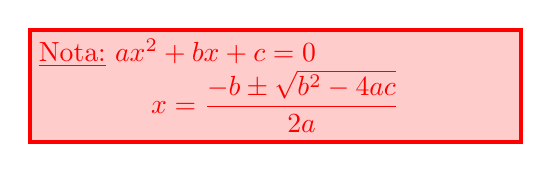
\begin{tikzpicture}
		\node[red, draw=red, fill=red!20, rectangle, line width=1.5pt, text width=6cm] {\underline{Nota:} $ax^2+bx+c=0$ \begin{center}
				$x=\dfrac{-b\pm\sqrt{b^2-4ac}}{2a}$
		\end{center}};
	\end{tikzpicture}
\end{wrapfigure}

$x^2-5x+6=0$

$x=\dfrac{5\pm\sqrt{25-4\cdot6}}{2\cdot 1}\left\{\begin{array}{l}
	\frac{5-1}{2}=3\\
	\frac{5-1}{2}=2
\end{array}\right.$

\begin{itemize}[label=\color{red}\textbullet, leftmargin=*]
	\item \color{lightblue} Proposiciones
\end{itemize}
Sentencia enunciada de la que se puede decir si es verdad o miente:
\begin{itemize}[label=\color{lightblue}$\rightarrow$]
	\item Está lloviendo \qquad 0 \textcolor{red}{(Falso)}
	\item La sangre es roja \quad 1\textcolor{olive}{(Verdadero)}
\end{itemize}
\begin{itemize}[label=\color{red}\textbullet, leftmargin=*]
	\item \color{lightblue} Proposiciones simples
\end{itemize}
Las proposiciones se escriben  con letras minúsculas: $p,q,r,s,t,\hdots$

Operaciones básicas lógicas:
\begin{itemize}[label=$-$]
	\item Disyunción $\vee$ "o"
	\item Conjunción $\wedge$ "y"
	\item Negación $\neg $ "no"
\end{itemize}
\begin{itemize}[label=\color{red}\textbullet, leftmargin=*]
	\item \color{lightblue}Tablas de verdad
\end{itemize}

	\begin{tabular}{|c|c|c|}
		\hline
		\rowcolor{lightblue!50}
		\hline
		$p$ & $q$ & $p\vee q$ \\ \hline
		1   & 1   & 1         \\ \hline
		1   & 0   & 1         \\ \hline
		0   & 1   & 1         \\ \hline
		0   & 0   & 0         \\ \hline
	\end{tabular}\qquad
	\begin{tabular}{|c|c|c|}
		\hline
		\rowcolor{lightblue!50}
		\hline
		$p$ & $q$ & $p\wedge q$ \\ \hline
		1   & 1   & 1           \\ \hline
		1   & 0   & 0           \\ \hline
		0   & 1   & 0           \\ \hline
		0   & 0   & 0           \\ \hline
	\end{tabular}\qquad
\begin{tabular}{|c|c|}
	\hline
	\rowcolor{lightblue!50}
	\hline
	$p$ & $\neg p$ \\ \hline
	1   & 0        \\ \hline
	0   & 1        \\ \hline
\end{tabular}
\pagebreak
\begin{wrapfigure}[4]{r}{0.4 \linewidth}
	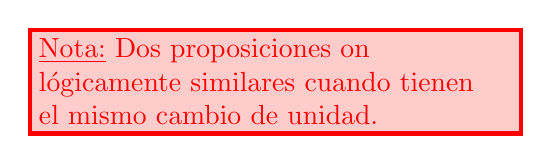
\begin{tikzpicture}[baseline=(current bounding box.center)]
		\node[red, draw=red, fill=red!20, line width=1.5pt, text width=6cm] {\underline{Nota:} Dos proposiciones on lógicamente similares cuando tienen el mismo cambio de unidad.};
	\end{tikzpicture}
\end{wrapfigure}

Orden de prioridad
\begin{enumerate}[label=\arabic*)]
	\item Negación
	\item Conjunción
	\item Disyunción
\end{enumerate}
\textcolor{lightblue}{\underline{Ejemplo}}

{\color{lightblue}$(p\vee q)\wedge r\renewcommand{\CancelColor}{\color{black}}\cancel{\equiv}p\vee q\wedge r$}

\begin{tabular}{|c|c|c|c|c|c|c|}
	\hline
	\rowcolor{lightblue!50}
	\hline
	$p$ & $q$ & $r$ & $p\vee q$ & $(p\vee q)\wedge r$ & $q\wedge r$ & $p\vee q\wedge r$ \\ \hline
	1   & 1   & 1   & 1         & 1                   & 1           & 1                 \\ \hline
	1   & 1   & 0   & 1         & 0                   & 0           & 1                 \\ \hline
	1   & 0   & 1   & 1         & 1                   & 0           & 1                 \\ \hline
	1   & 0   & 0   & 1         & 0                   & 0           & 1                 \\ \hline
	0   & 1   & 1   & 1         & 1                   & 1           & 1                 \\ \hline
	0   & 1   & 0   & 1         & 0                   & 0           & 0                 \\ \hline
	0   & 0   & 1   & 0         & 0                   & 0           & 0                 \\ \hline
	0   & 0   & 0   & 0         & 0                   & 0           & 0                 \\ \hline
\end{tabular}

{\color{lightblue}$\neg p\vee q r\renewcommand{\CancelColor}{\color{black}}\cancel{\equiv}\neg(p\vee q)$}

\begin{tabular}{|c|c|c|c|c|c|}
	\hline
	\rowcolor{lightblue!50}
	\hline
	$p$ & $q$ & $\neg p$ & $\neg p\vee q$ & $p\vee q$ & $\neg (p\vee q)$ \\ \hline
	1   & 1   & 0        & 1              & 1         & 0                \\ \hline
	1   & 0   & 0        & 0              & 1         & 0                \\ \hline
	0   & 1   & 1        & 1              & 1         & 0                \\ \hline
	0   & 0   & 1        & 1              & 0         & 1                \\ \hline
\end{tabular}
\pagebreak

{\color{lightblue}$\neg(p\vee q)\equiv\neg p\vee\neg p$}

\begin{tabular}{|c|c|c|c|c|c|}
	\hline
	\rowcolor{lightblue!50}
	\hline
	$p$ & $q$ & $\neg p$ & $\neg q$ & $\neg p\vee \neg q$ & $\neg p\wedge \neg q$ \\ \hline
	1   & 1   & 0        & 0        & 1                   & 0                     \\ \hline
	1   & 0   & 0        & 1        & 0                   & 0                     \\ \hline
	0   & 1   & 1        & 0        & 1                   & 0                     \\ \hline
	0   & 0   & 1        & 1        & 1                   & 1                     \\ \hline
\end{tabular}
\begin{itemize}[label=\color{red}\textbullet]
	\item {\color{lightblue} Tautología: } La tabla de verdad tiene todo 1 $\quad(p\vee\neg p)$
	\item {\color{lightblue} Contradicción: } La tabla de verdad tiene todo 0 $\quad(p\wedge\neg p)$
\end{itemize}
\begin{itemize}[label=\color{red}\textbullet, leftmargin=*]
	\item \color{lightblue} Álgebra de porposiciones
\end{itemize}

\begin{tabular}{|c|c|c|}
	\hline
	\rowcolor{lightblue!50}
	\hline
	$p$ & 0 & $p\vee0$ \\ \hline
	1   & 0 & 1        \\ \hline
	0   & 0 & 0        \\ \hline
\end{tabular}\qquad\begin{tabular}{|c|c|c|}
\hline
\rowcolor{lightblue!50}
\hline
$p$ & 1 & $p\vee1$ \\ \hline
1   & 1 & 1        \\ \hline
0   & 1 & 1        \\ \hline
\end{tabular}

$\begin{array}{lll}
	p \vee 0 \equiv p & p \wedge 1 \equiv p & \multirow{3}{*}{\text{\color{lightblue} Leyes de identidad}} \\
	p \vee 1 \equiv 1 & p \wedge 0 \equiv 0 & \\
	p \vee p \equiv p & p \wedge p \equiv p & \\[1ex]
	p \vee (q \vee r) \equiv (p \vee q) \vee r & p \wedge (q \wedge r) \equiv (p \wedge q) \wedge r & \text{\color{lightblue} Leyes asociativas} \\[1ex]
	p \vee q \equiv q \vee p & p \wedge q \equiv q \wedge p & \text{\color{lightblue} Leyes conmutativas} \\[1ex]
	p \vee (q \wedge r) \equiv (p \vee q) \wedge (p \vee r) & p \wedge (q \vee r) \equiv (p \wedge q) \vee (p \wedge r) & \text{\color{lightblue} Leyes distributivas} \\[1ex]
	\neg \neg p \equiv p & & \text{\color{lightblue} Ley de doble negación} \\[1ex]
	\neg 1 \equiv 0~~p \vee \neg p \equiv 1 & \neg 0 \equiv 1~~p \wedge \neg p \equiv 0 & \text{\color{lightblue} Leyes de los complementos} \\[1ex]
	\neg (p \vee q) \equiv \neg p \wedge \neg q & \neg (p \wedge q) \equiv \neg p \vee \neg q & \text{\color{lightblue} Leyes de DeMorgan}
\end{array}$

\begin{itemize}[label=\color{red}\textbullet, leftmargin=*]
	\item \color{lightblue}Demostración
\end{itemize}
$\begin{array}{c}
	\neg(p\vee q)\vee(\neg p\wedge q)\equiv\neg p\\
	(\neg p\wedge\neg q)\vee(\neg p\wedge q)\\
	\neg p\wedge(\neg q\vee q)\\
	\neg p\wedge1\\
	\neg p
\end{array}$
\begin{itemize}[label=\color{red}\textbullet, leftmargin=*]
	\item \color{lightblue}Proposiciones
\end{itemize}
$\begin{array}{l}
	p\rightarrow q\\
	p\leftrightarrow q\\
	(p\rightarrow q)\wedge(q\rightarrow p)\\
	(\neg p\vee q)\wedge(\neg q\vee p)
\end{array}\qquad$
\begin{tabular}{|c|c|c|c|}
	\hline
	\rowcolor{lightblue!50}
	\hline
	$p$ & $q$ & $p\rightarrow q$ & $p\leftrightarrow q$ \\ \hline
	1   & 1   & 1                & 1                    \\ \hline
	1   & 0   & 0                & 0                    \\ \hline
	0   & 1   & 1                & 0                    \\ \hline
	0   & 0   & 1                & 1                    \\ \hline
\end{tabular}

$\begin{array}{ll}
	p\rightarrow q\equiv\neg p\vee q & p\rightarrow q\equiv\neg q\rightarrow\neg p\\
	\begin{tabular}{|c|c|c|c|}
		\hline
		\rowcolor{lightblue!50}
		\hline
		$p$ & $q$ & $\neg p$ & $\neg p\vee q$ \\ \hline
		1   & 1   & 0        & 1              \\ \hline
		1   & 0   & 0        & 0              \\ \hline
		0   & 1   & 1        & 1              \\ \hline
		0   & 0   & 1        & 1              \\ \hline
	\end{tabular} & \begin{tabular}{|c|c|c|c|c|}
	\hline
	\rowcolor{lightblue!50}
	\hline
	$p$ & $q$ & $\neg p$ & $\neg q$ & $\neg p\rightarrow\neg q$ \\ \hline
	1   & 1   & 0        & 0        & 1                         \\ \hline
	1   & 0   & 0        & 1        & 0                         \\ \hline
	0   & 1   & 1        & 0        & 1                         \\ \hline
	0   & 0   & 1        & 1        & 1                         \\ \hline
	\end{tabular}\\
	 
\end{array}$
\begin{itemize}[label=\color{red}\textbullet, leftmargin=*]
	\item \color{lightblue}Deducciones lógicas
\end{itemize}
Si $n$ es natural entonces $2n$ es par.

Si $a,b,c\in\mathbb{R}$ y $a\neq0$ entonces la solución de $ax`2+bx+c=0$ es $x=\dfrac{-b\pm\sqrt{b^2-4ac}}{2a}$

$\{p_1,p_2,p_4\}\rightarrow q$

$\{p_1,p_2,\hdots,p_n\}\rightarrow q\qquad p_1\wedge p_2\wedge\cdots\wedge p_n\rightarrow q$ es tautología, si no es una falacia.

\pagebreak

$\{p\rightarrow q,p\}\rightarrow q$

\begin{tabular}{|c|c|c|c|c|}
	\hline
	\rowcolor{lightblue!50}
	\hline
	$p$ & $q$ & $p\rightarrow q$ & $(p\rightarrow q)\wedge p$ & $\left((p\rightarrow q)\wedge p\right)\rightarrow q$ \\ \hline
	1   & 1   & 1                & 1                          & 1                                                    \\ \hline
	1   & 0   & 0                & 0                          & 1                                                    \\ \hline
	0   & 1   & 1                & 0                          & 1                                                    \\ \hline
	0   & 0   & 1                & 0                          & 1                                                    \\ \hline
\end{tabular}

$\{p\rightarrow q,q\}\rightarrow p$

\begin{tabular}{|c|c|c|c|c|}
	\hline
	\rowcolor{lightblue!50}
	\hline
	$p$ & $q$ & $p\rightarrow q$ & $(p\rightarrow q)\wedge q$ & $\left((p\rightarrow q)\wedge q\right)\rightarrow p$ \\ \hline
	1   & 1   & 1                & 1                          & 1                                                    \\ \hline
	1   & 0   & 0                & 0                          & 1                                                    \\ \hline
	0   & 1   & 1                & 1                          & 0                                                    \\ \hline
	0   & 0   & 1                & 0                          & 1                                                    \\ \hline
\end{tabular}

$\{p\rightarrow q,q\rightarrow r\}\rightarrow (p\rightarrow r)$

\begin{tabular}{|c|c|c|c|c|c|c|c|}
	\hline
	\rowcolor{lightblue!50}
	\hline
	$p$ & $q$ & $r$ & $p\rightarrow q$ & $q\rightarrow r$ & $(p\rightarrow q)\wedge(q\rightarrow r)$ & $p\rightarrow r$ & $\left((p\wedge q)\wedge(q\rightarrow r)\right)\rightarrow(p\rightarrow r)$ \\ \hline
	1   & 1   & 1   & 1                & 1                & 1                                        & 1                & 1                                                                           \\ \hline
	1   & 1   & 0   & 1                & 0                & 0                                        & 0                & 1                                                                           \\ \hline
	1   & 0   & 1   & 0                & 1                & 0                                        & 1                & 1                                                                           \\ \hline
	1   & 0   & 0   & 0                & 1                & 0                                        & 0                & 1                                                                           \\ \hline
	0   & 1   & 1   & 1                & 1                & 1                                        & 1                & 1                                                                           \\ \hline
	0   & 1   & 0   & 1                & 0                & 0                                        & 1                & 1                                                                           \\ \hline
	0   & 0   & 1   & 1                & 1                & 1                                        & 1                & 1                                                                           \\ \hline
	0   & 0   & 0   & 1                & 1                & 1                                        & 1                & 1                                                                           \\ \hline
\end{tabular}
\begin{itemize}[label=\color{red}\textbullet, leftmargin=*]
	\item \color{lightblue}Lógica de propiedades
\end{itemize}
\begin{wrapfigure}[4]{r}{0.4\linewidth}
	\begin{tikzpicture}[framed, baseline=(current bounding box.center)]
		\begin{axis}[
			ymin=0,
			xmin=0,
			ymax=9.5,
			xmax=3.5,
			xlabel=$n$,
			axis lines=center,
			]
			\addplot[color=lightblue, domain=0:3.5, samples=150] {x^2};
		\end{axis}
	\end{tikzpicture}
\end{wrapfigure}

Si $n\ge 3$ entonces $n^2>4$.

$\mathbb{N}=\{1,2,3,\hdots\}\qquad P(n)=n^2>4\left\{\begin{array}{ll}
	P(1)=1>4 & \textcolor{lightblue}{0}\\
	P(2)=4>4 & \textcolor{lightblue}{0}\\
	P(3)=9>4 & \textcolor{lightblue}{1}
\end{array}\right.$

$-$ Conjunto de verdad: conjunto de elementos que verifica $P(n)$.

$P(n,m)\qquad T_P=\{(1,1), (1,2),(2,1),(2,2)\}$

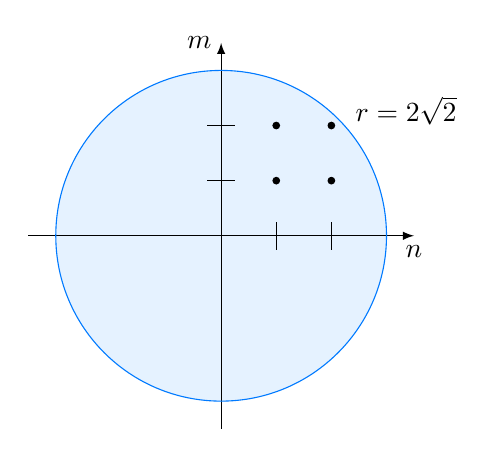
\begin{tikzpicture}[>=latex, scale=0.7]
	\fill[fill=lightblue!10] (0,0) circle (3);
	\draw[->] (-3.5,0) -- (3.5,0) node[below] {$n$};
	\draw[->] (0,-3.5) -- (0,3.5) node[left] {$m$};
	\draw[draw=lightblue] (0,0) circle (3) node[right] at (45:3.2) {$r=2\sqrt{2}$};
	\foreach \x/\y in {1/1, 1/2, 2/1, 2/2} {	
		\fill (\x,\y) circle (2pt);
		\draw (\x, -0.25) -- (\x,0.25);
		\draw (-0.25,\y) -- (0.25,\y);
		}
\end{tikzpicture}


$\begin{array}{ll}
		n,m\in\mathbb{N},\qquad& P(n)~~n^2<4\qquad T_P=\{1\}\\
	 & Q(m),~2m\ge3\qquad T_Q=\{2,4,\hdots\}\\
	 & \left[\exists nP(n)\right]\wedge\left[\forall mQm\right] \text{ es }0\\
	 & \left[\exists nP(n)\right]\vee\left[\forall mQm\right] \text{ es }1\\
	 & \neg\left[\exists nP(n)\right]\wedge\left[\forall mQm\right] \text{ es }0\\
\end{array}$\hspace{2cm}
\fcolorbox{lightblue}{lightblue!10}{$\begin{array}{l}
		\neg\left(\exists nP(n)\right)\equiv\forall n\neg P(n)\\
		\neg\left(\forall nP(n)\right)\equiv\exists n\neg P(n)
	\end{array}$}

$\begin{array}{ll}
	\exists n\exists mP(n,m)\text{ es }1\qquad~~ & \forall n\forall m\neg\left(P(n,m)\right)\equiv\neg\left(\exists n\exists mP(n,m)\right)\\
	\forall n\forall mP(n,m)\text{ es }0 & \exists n\exists m\neg\left(P(n,m)\right)\equiv\neg\left(\forall n\forall mP(n,m)\right)\\
	\exists n\forall mP(n,m)\text{ es }0 & \forall n\exists m\neg\left(P(n,m)\right)\equiv\neg\left(\exists n\forall mP(n,m)\right)\\
	\forall n\exists mP(n,m)\text{ es }1 & \exists n\forall m\neg\left(P(n,m)\right)\equiv\neg\left(\forall n\exists mP(n,m)\right)\\
\end{array}$

\begin{itemize}[label=\color{red}\textbullet, leftmargin=*]
	\item \color{lightblue}Ejercicios 26/09/23
\end{itemize}
\textcolor{red}{17) }\textcolor{lightblue}{$\left[(p\wedge q)\longleftrightarrow(\vee\neg r)\right]\vee p$}

$(\neg p\vee q)\wedge(\neg q\vee p)\equiv\left((\neg p\vee q)\wedge\neg q\right) \vee\left((\neg p\vee q)\wedge p\right)\equiv\overbrace{(\neg p\wedge\neg q\vee\underbrace{q\wedge \neg q}_{0})}^{\neg p\wedge\neg q\equiv\neg(p\vee q)}\vee(\overbrace{\underbrace{\neg p\wedge p}_{0}\vee p\wedge q}^{p\wedge q})$

\begin{center}
	\begin{tabular}{|c|c|c|c|c|c|c|c|}
		\hline
		\rowcolor{lightblue!50}
		\hline
		$p$ & $q$ & $r$ & $\neg r$ & $p\wedge q$ & $p\vee\neg r$ & $(p\wedge q)\longleftrightarrow (p\vee\neg r)$ & $[(p\wedge q)\longleftrightarrow (p\vee\neg r)]\vee p$ \\
		\hline
		1 & 1 & 1 & 0 & 1 & 1 & 1 & 1 \\
		\hline
		1 & 1 & 0 & 1 & 1 & 1 & 1 & 1 \\
		\hline
		1 & 0 & 1 & 0 & 0 & 1 & 0 & 1 \\
		\hline
		1 & 0 & 0 & 1 & 0 & 1 & 0 & 1 \\
		\hline
		0 & 1 & 1 & 0 & 0 & 1 & 0 & 0 \\
		\hline
		0 & 1 & 0 & 1 & 0 & 0 & 1 & 1 \\
		\hline
		0 & 0 & 1 & 0 & 0 & 1 & 0 & 0 \\
		\hline
		0 & 0 & 0 & 1 & 0 & 0 & 1 & 1 \\
		\hline
	\end{tabular}
\end{center}

\newpage

\textcolor{red}{Tema 2: Conjuntos}	

Un conjunto es una colección de objetos (elementos).

$a\in A$

$\begin{array}{ll}
	\mathbb{N}=\{1,2,\hdots\} & A=\{1,2,3\}=\{n\in\mathbb{N}:n<4\}\\
	\mathbb{Z}=\{\hdots,-2,-1,0,1,2,\hdots\} & B=\{n\in\mathbb{N}:n>4\}=\{5,6,\hdots\}
\end{array}$

Dados $A$ y $B$ conjuntos:
\begin{itemize}
	\item[] $A\subseteq B$ si $\forall~a\in A$ se cumple que $a\in B$
	\item[] $A=B$ si $A\subseteq B$ y $B\subseteq A$
\end{itemize}
$A\subsetneq B$ (no está contenido).

$A\neq B$ (es distinto de).

Si $A\subseteq B$ y $A\neq B\longrightarrow A\subsetneq B$

Diagrama de Venn.

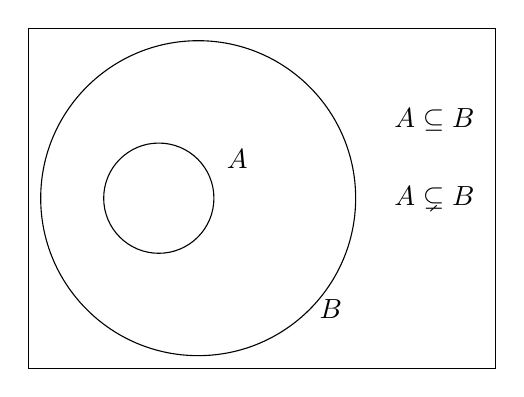
\begin{tikzpicture}[baseline=(current bounding box.center), framed]
	\draw (0,0) circle (2) ;
	\draw (-0.5,0) circle (0.7) ;
	\node (A) at (320:2.2) { $B$};
	\node (A) at (45:0.7) { $A$};
	\node at (3, 1) {$A\subseteq B$};
	\node at (3, 0) {$A\subsetneq B$};
\end{tikzpicture}\hspace{0.7cm}
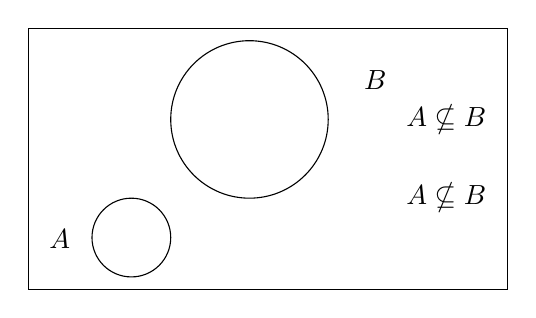
\begin{tikzpicture}[baseline=(current bounding box.center), framed]
	\draw (1,1) circle (1) node at (30:3) {$B$};
	\draw (-0.5,-0.5) circle (0.5) node at (200:1.5) {$A$};
	\node at (3.5,1) {$A\nsubseteq B$};
	\node at (3.5,0) {$A\nsubseteq B$};
\end{tikzpicture}\hspace{0.7cm}
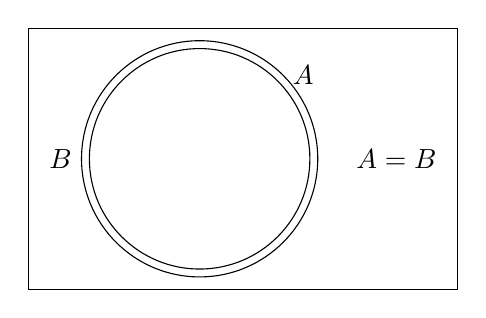
\begin{tikzpicture}[baseline=(current bounding box.center), framed]
	\draw (0,0) circle (1.5) node[left] at (180:1.5) {$B$};
	\draw (0,0) circle (1.4) node[right] at (45:1.5) {$A$};
	\node at (2.5,0) {$A=B$};
\end{tikzpicture}

\textcolor{lightblue}{\underline{Operaciones}}

\begin{itemize}
	\item Intersección: $A\cap B=\{x:x\in A\wedge x\in B\}$
	\item Unión: $A\cup B=\{x:x\in A\vee x\in B\}$
	\item Complementario: $A^c=\{x\in\mathrm{U}:\underset{\neg(x\in A)}{x\notin A}\}$
\end{itemize}
\begin{wrapfigure}[4]{l}{0.3 \linewidth}
	\begin{venndiagram2sets}[shade=lightblue!50]
	\fillACapB
\end{venndiagram2sets}
\end{wrapfigure}

	$A\cup B=\varnothing \qquad A\cup\mathrm{U}\text{ Conjunto universal }=A$
	
	$A\cup\varnothing=A $
	
	$A\cap\varnothing=\varnothing $
\newline


\textcolor{lightblue}{\underline{Álgebra de conjuntos}}
\begin{itemize}
	\item Leyes idempotentes $\quad A\cup A=A\quad A\cap A=A$
	\item Leyes asociativas $\quad A\cup(B\cup C)=(A\cup B)\cup C\quad A\cap(B\cap C)=(A\cap B)\cap C$
	\item Leyes conmutativas $\quad A\cup B=B\cup A\quad A\cap B=A\cap B$
	\item Leyes distributivas$\quad A\cup(B\cap C)=(A)\cap B)\cup(A\cap C) \quad A\cap(B\cup C)=(A)\cup B)\cap(A\cup C) $
	\item Leyes de identidad $\quad A\cup \varnothing=A~~A\cup\mathrm{U}=\mathrm{U}\quad A\cap\varnothing=\varnothing~~A\cap\mathrm{U}=A$
	\item Leeys de involución $\quad(A^c)^c=A$
	\item Leyes de complementos $\quad A\cup A^c=\mathrm{U}~~\mathrm{U}^c=0\quad A\cap A^c=\varnothing~~\varnothing^c=\mathrm{U}$
	\item Leyes de DeMorgan $\quad(A\cup B)^c=A^c\cap B^c\quad(A\cap B)^c=A^c\cup B^c$
\end{itemize}
\begin{wrapfigure}[4]{l}{0.27\textwidth}
	\begin{venndiagram2sets}[shade=lightblue!50]
	\fillNotAorB
\end{venndiagram2sets}
\end{wrapfigure}

	$(A\cup B)^c=A^c\cap B^c$
	
	$(A\cup B)^c=A^c\cap B^c$
	
	$A^c\cap B^c\subseteq(A\cup B)^c$
	
	$x\in(A\cup B)^c\rightarrow x\notin A\cup B\rightarrow x\notin A\wedge x\notin B\equiv x\in A^c,~x\in 
	B^c\rightarrow x\in A^c\cap B^c$

\textcolor{lightblue}{\underline{Diferencia}}

$A\backslash B=\{x\in\mathrm{U}:x\in A\wedge x\notin B\}\equiv A\cap B^c$

$A^C=\mathrm{U}\backslash A$

$\begin{array}{l}
	A=\{1,2\}\\
	B=\{2,3\}\\
	\underset{\{4\}}{A\backslash B}\neq\underset{\{3\}}{B\backslash A}
\end{array}$

$a,A,\subseteq,=,\cap,\cup,\backslash,A^c$


{\color{lightblue}\underline{Principio de inducción-exclusión}}

Dado $A$ conjunto, $|A|$ es el número de elementos de $A$.

Si $A,~B$ son finitos, entonces $|A\cup B|=|A|-|B|-|A\cap B|$

\begin{itemize}[label=\color{red}\textbullet, leftmargin=*]
	\item \color{lightblue}Demostración
\end{itemize}
\begin{wrapfigure}[2]{l}{0.2\textwidth}
	\begin{venndiagram2sets}[shade=lightblue!50, tikzoptions={scale=0.7}]
		\fillACapB
	\end{venndiagram2sets}
\end{wrapfigure}

Caso 1. $A\cap B=\varnothing\longrightarrow|A\cup B|=|A|+|B|$

Caso 2. $A\cap B\neq\varnothing\qquad A\cup B=\underset{\displaystyle A\cap (B\backslash A)=\varnothing}{A\cup(B\backslash A)}\longrightarrow|A\cup B|=|A|+|B\backslash A|$\newline

\begin{itemize}[label=\color{red}\textbullet, leftmargin=*]
	\item \color{lightblue} Ejemplo
\end{itemize}
50 alumnos 

28 tienen IPHONE $|A|=28\qquad|A\cap B|=28+33-50=5$ \\
20 tiene el MALO CARO $|B|=20$\\
13 tienen el MALO BARATO $|C|=13\qquad|A\cup B\cup C|=50$

$|A\cap B\cap C|=?$

$\begin{array}{ll}
	|(A\cup B)\cup C|&=|A\cup B|+|C|-|(A\cup B)\cap C|\\
	&=|A|+|B|-|A\cap B|+|C|-(|A\cap C|+|B\cap C|-\underset{C\cap C=C}{\overbrace{A\cap C\cap B\cap C}^{A\cap B\cap C}}|)\\
	&=|A|+|B|+|C|-|A\cap B|-|A\cap C|-|B\cap C|+|A\cap B\cap C|=|A\cup B\cup C|\\
	& 50=28+20+13-7-5-4+|A\cap B\cap C|\longrightarrow|A\cap B\cap C|=5
\end{array}$

\textcolor{lightblue}{\underline{Relaciones}}

$A,~B\longrightarrow$ producto cartesiano \[ A\times B=\{(a,b):a\in A,b\in B\} \] $\begin{array}{l}
	A=\{1,2\}\\
	B=\{3,4\}
\end{array}\qquad R=\{(1,3),(1,4),(2,3),(2,4)\}$

Si $A$ y $B$ son finitos $\longrightarrow|A\times B|=|A|\cdot |B|$

Si $A=B\longrightarrow A\times A=A^2$

Una relación $\sim$ es un subconjunto de $A\times B$.

Si $A=B,~\sim$ es una relación sobre $A$.

\begin{itemize}[label=\color{red}\textbullet, leftmargin=*]
	\item \color{lightblue}Ejemplos
\end{itemize}
$R=\{(2,3). (2,4)\}\qquad\begin{array}{l}
	2\sim 3\\
	1\nsim 3
\end{array}$

$R^2=R\times R$

$f(x)=x^2$

Una función es una relación  $R$ en $A\times B$ de manera que que $\forall a\in A$

$\exists$ un único $b\in B$ tal que $\underset{\displaystyle a\sim b}{(a,b)\in R}\longleftrightarrow $ Si $(a,b_1)\in R$ y $(a,b_2)\in R\longrightarrow b_1=b_2$

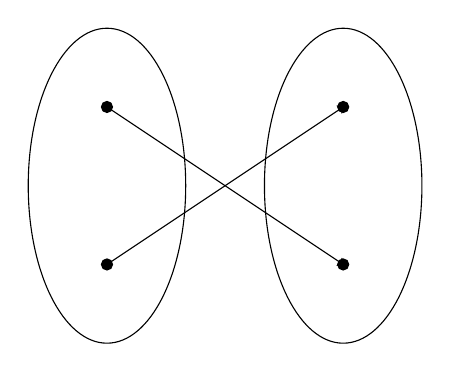
\begin{tikzpicture}[baseline=(current bounding box.center)]
	\draw (0,0) ellipse (1cm and 2cm);
	\draw (3,0) ellipse (1cm and 2cm);
	\filldraw (0,1) circle (2pt);
	\filldraw (0,-1) circle (2pt);
	\filldraw (3,1) circle (2pt);
	\filldraw (3,-1) circle (2pt);
	\draw[->] (0,-1) -- (3,1);
	\draw[->] (0,1) -- (3,-1);
\end{tikzpicture}

Sea $R$ relación sobre $A$. $(R\subseteq A\times A)$

$R$ puede ser:
\begin{enumerate}[label=\arabic*)]
	\item Reflexiva si $a\sim a\quad\forall a\in A$.
	\item Simétrica si $\forall a_1,a_2\in A$ tal que $a_1\sim a_2$ se cumple que $a_2\sim a_1$.
	\item Antisimétria si $\forall a_1,a_2\in A$ tal que $a_1\sim a_2~(a_1\sim a:2 \wedge a_2\sim a_1\longrightarrow a_1=a_2)$ se cumple que $a_2\nsim a_1$
	\item Transitiva si $\forall a_1,a_2,a_3\in A$ tal que $a_1\sim a_2$ y $a_2\sim a_2$ tal que $a_1\sim a_3$.
\end{enumerate}
\textcolor{lightblue}{\underline{Relación de equivalencia}}

Una relación $R$ sobre un conjunto $A\neq\varnothing$ es de equivalencia  si es:
\begin{itemize}[label=$-$]
	\item Reflexiva $a\sim a~\forall a\in A$
	\item Simétrica si $a\sim b\rightarrow b\sim a~\forall a,b\in A$
	\item Transitiva si $a\sim b$ y $b\sim c\rightarrow a\sim c~\forall a,b,c\in A$
\end{itemize}
\begin{itemize}[label=\color{red}\textbullet, leftmargin=*]
	\item \color{lightblue}Ejemplos
\end{itemize}
\begin{enumerate}[label=\color{lightblue}\arabic*)]
	\item $\mathbb{N}~n\sim m$ si $n-m$ es par
	
	Reflexiva $n\sim n~~n-n=0$ es par
	
	Simétrica $n\sim m\rightarrow n-m$ es par $\rightarrow m-n$ es par $\rightarrow m\sim n$.
	
	$\begin{array}{ll}
		\text{Transitiva } & n\sim m\rightarrow n-m \text{ es par }\qquad \underbrace{n-m}+\underbrace{m-\tilde{n}}=n-\tilde{n} \text{ es par }\rightarrow n\sim \tilde{n}\\
		 & m\sim \tilde{n}\rightarrow m-\tilde{n}\text{ es par } 
	\end{array}$
\end{enumerate}
\begin{itemize}[label=\color{red}\textbullet, leftmargin=*]
	\item \color{lightblue}Clases de equivalencia
\end{itemize}
$a\in A\qquad [a]:=\{b\in A:a\sim b\}$
\begin{enumerate}[label=\arabic*)]
	\item Teorema
\end{enumerate}
$R$ relación de equivalencia entre $A\neq0~\forall a,b\in A$ o bien $\underbrace{[a]=[b]}_{\displaystyle a\sim b}$ o bien $\underbrace{[a]\cap[b]=\varnothing}_{\displaystyle a\nsim b}$.
\begin{itemize}[label=\color{red}\textbullet, leftmargin=*]
	\item \color{lightblue}Demostración
\end{itemize}
Sea $a,b\in A,~a\neq b\left\lbrace\begin{array}{l}
	a\sim b\\
	a\nsim b
\end{array}\right.$

$a\sim b\rightarrow ¿[a]=[b] ?$

$[a]\subseteq[b]$. Sea $x\in[a]\rightarrow\left.\begin{array}{l}
	a\sim c\\
	b\sim a
\end{array}\right\}\rightarrow b\sim c\rightarrow c\in[b]$

$a\nsim b$ Reducción al absurdo. $(p\to q\equiv\neg q\to\neg p)$

Sea $c\in[a]\cap[b]\neq\varnothing\rightarrow\left.\begin{array}{l}
	c\in[a]\rightarrow a\sim c\\
	c\in[b]\rightarrow b\sim c\rightarrow c\sim b
\end{array} \right\}\rightarrow a\sim b$

\textcolor{lightblue}{\underline{Relación de Orden}}

Una relación $R$ sobre $A\neq\varnothing$ se dice de orden si cumple.
\begin{itemize}
	\item Relación reflexiva
	\item Relación transitiva
	\item Relación antisimétrica. Si $a\sim b\rightarrow b\nsim a~\forall a,b\in A$.
\end{itemize}
\begin{itemize}[label=\color{red}\textbullet, leftmargin=*]
	\item \color{lightblue}Ejemplo
\end{itemize}
$\mathbb{N}\qquad n\le m$ si $n$ divide $m.~(n|m)\leftrightarrow\exists k\in\mathbb{N}$ tal que {\color{lightblue}$n\cdot k=m$}
\begin{itemize}[leftmargin=*]
	\item Reflexiva: $n\cdot 1=n\rightarrow n|n\rightarrow n\le n$.
	
	$ \begin{array}{ll}
		\bullet~~\text{Antisimétrica: } & n\le m\rightarrow n|m\rightarrow\exists k_1\in\mathbb{N} \text{ tal que }n\cdot k_1=m\\
		& m\le n\rightarrow m|n\rightarrow\exists k_2\in\mathbb{N} \text{ tal que }m\cdot k_2=n\\
		& \qquad m\cdot k_1\cdot k_2=m\rightarrow k_1,k_2=1\rightarrow k_1=k_2=1
	\end{array}$
	
	$\left.\begin{array}{ll}
		\bullet~~\text{Transitiva:} & n\le m\rightarrow\exists k_1\in\mathbb{N}\text{ tal que } n\cdot k_1=m\\
		& n\le\tilde{n}\rightarrow\exists k_2\in\mathbb{N}\text{ tal que }m\cdot k_2=\tilde{n}
	\end{array}\right\}\rightarrow n\underset{\in\mathbb{N}}{(k_1\cdot k_2)}=\tilde{n}\rightarrow n|\tilde{n}\rightarrow n\le \tilde{n}$
\end{itemize}
Relación de orden parcial

$(\mathbb{N},\underset{
\text{orden usual}
}{\le})$ Relación de orden total

$n\le m \leftrightarrow \exists k\in\mathbb{N}\cup\{0\}$ tal que $n+k=m$

Una relación $R$ sobre $A\neq\varnothing$ y $A$ finito.

Diagramas de Hasse

$A=\{1,2,3,4,5\}$

$R=\{(1,1),(1,2)\overset{(1,3)}{,}(1,4)\overset{(1,5)}{,}(2,2),(2,3)\overset{(2,5)}{,}(3,3),(3,5),(4,4),(5,5),(4,5)\}$

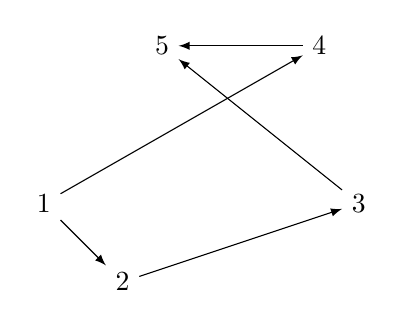
\begin{tikzpicture}[baseline=(current bounding box.center), >=latex]
	\node (1) at (0,0) {1};
	\node (2) at (1,-1) {2};
	\node (3) at (4,0) {3};
	\node (4) at (3.5, 2) {4};
	\node (5) at (1.5, 2) {5};
	\draw[->] (1) -- (2);
	\draw[->] (2) -- (3);
	\draw[->] (1) -- (4);
	\draw[->] (4) -- (5);
	\draw[->] (3) -- (5);
\end{tikzpicture}$\qquad\left.\begin{array}{c}
1\le 2\\
2\le 3
\end{array}\right\}\rightarrow 1\le 3$

Relación de orden sobre $A\neq\varnothing\qquad B\subseteq A$ 

$a\in A$\\
$a$ es supremo de $B$ si $b\le a~\forall b\in B$\\
$a$ es cota inferior de $B $ si $a\le b~\forall b\in B$\\
$a$ es supremo de $B$ si es la menor cota superior\\
$a$ es ínfimo de $B$ si es la myor cota inferior\\
$a$ es máximo de $B$ si es supremo de $B$ y $a\in B$
$a$ es mínimo de $B$ si es ínfimo de $B$ y $a\in B$

$A=\{1,2,3,4,5,6,9,12\}~n\le m$ si $n|m$ \\
$B=\{1,2,3\}$

Cota superior $=\{6, 12\}$

{\renewcommand{\arraystretch}{1} $\begin{array}{l}
	b\in B\text{ es maximal si }\\
	\nexists a\in B \text{ tal que } b\le a\\
	b\in a\text{ es minimal si }\\
	\nexists a\in B\text{ tal que }a\le b 
\end{array}\leftarrow \begin{array}{l}
\text{Elemento} \\
\text{maximal}
\end{array}\rightarrow$\fbox{C.S}$\rightarrow S\rightarrow\max$}

\textcolor{lightblue}{\underline{Principio de inducción}}

$1+3+5+\cdots+2n-1=n^2$

{\renewcommand{\arraystretch}{1}$\begin{array}{l}
	1\\
	1+1=2\\
	2+1=3\\
	3+1=4\\
	\vdots\\
	\qquad=n\\
	n+1
\end{array}\qquad \begin{array}{l}
\mathbb{N}=P(n)=\{n\in\mathbb{N}:1+3+5+\cdots+2n-1=n^2\text{ es V}\}\\
\qquad\bullet\quad1\in P(m).\qquad1=1^2\\
\qquad\bullet\quad \text{Si }n\in P(m)\rightarrow n+1\in P(m)\qquad \text{\textquestiondown} 1+3+\cdots+\underset{2(n+1)-1}{2n+1}=(n+1)^2?\\
\underbrace{1+3+5+\cdots+2n-1}+2n+1=n^2+2n+1=(n+1)^2 
\end{array}$} 

\begin{itemize}[label=\color{red}\textbullet, leftmargin=*]
	\item \color{lightblue}Ejercicios 27/09/2023
\end{itemize}
\textcolor{red}{28)}

$X=\{1,2,3,4,5\}$
\begin{enumerate}[label=\color{red}\alph*)]
	\item $(\exists x(x+3=18))\equiv \forall x(x+3\neq10)$
	\item $\forall x(x+3<10)$ es 1
	\item $\exists x(x+3<10)$ es 1
	\item $\forall x(x+3\le 7)$ es 0 $\exists x(x+3>7)$ es 1
\end{enumerate}
\textcolor{red}{29)}

$X=\{1,2,3\}$
\begin{enumerate}[label=\color{red}\alph*)]
	\item $\exists x\forall y(x^2<y+1)\qquad x=1\qquad 1<y+1$
	\item $\forall x\exists y(x^2+y^2<12)$
	
	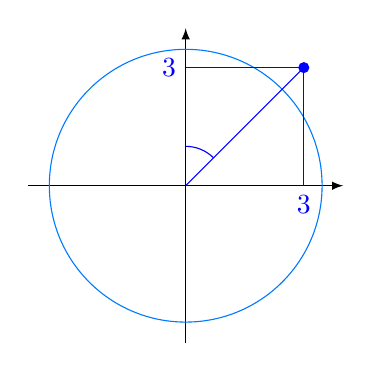
\begin{tikzpicture}[scale=0.5]
		\draw[-latex] (-4,0) -- (4,0);
		\draw[-latex] (0,-4) -- (0,4);
		\draw[lightblue] (0,0) circle (3.464);
		\draw[blue] (0,0) -- (3,3);
		\draw[blue] (0,3) node[left] {3} -- (3,3) -- (3,0) node[below] {3};
		\draw[blue] (0,1) arc (90:45:1) ;
		\fill[blue] (3,3) circle (4pt);
	\end{tikzpicture}
	\item $\neg(\forall x\forall y(x^2+y^2<12))\equiv \exists x\exists y(x^2+y^2<12)$
\end{enumerate}
\textcolor{red}{31)} $\exists x P(x)\wedge Q(x)$
\begin{enumerate}[label=\color{red}\alph*)]
	\item $\forall x P(x)\longleftrightarrow Q(x)$ es 1 $\begin{array}{ll}
		\nearrow & \forall x\neg P(x)\wedge\neg Q(x)\qquad (P(x)\text{ y }Q(x) \text{ sean falsa})\\
		\searrow & \exists x P(x)\wedge Q(x)
	\end{array}$
	\item $P(a)\vee Q(b)\equiv\exists a\exists b\quad P(a)\vee Q(b)$
\end{enumerate}
\textcolor{red}{32) }$\exists xQ(x)\equiv\forall xQ(x)$
\begin{enumerate}[label=\color{red}\alph*)]
	\item $\forall x\exists y P(y)\rightarrow Q(x)$
	\item $P(a)\vee Q(b)$
\end{enumerate}
\newpage
\includepdf[pages=-]{"G:/Mi Unidad/Goodnotes/1º Curso/1º Cuatrimestre/Matemática Discreta/Tema 3- Grafos.pdf"}
\textcolor{red}{Tema 4: Aritmética (modular)}

$(\mathbb{Z, +,\cdot})$ Anillo
\begin{itemize}
	\item[$+$] Asociativa, comunicativa, elemento neutro (0), elemento $\overset{\displaystyle\text{inverso}}{\text{simétrico}}$ $(\overset{n-n}{n+(-n)}=0)$ 
	\item[$\cdot$] Asociativa, comunicativo, elemento neutro (1), distributivo respecto de la suma $n\cdot(m+\tilde{n})=n\cdot m+n\cdot\tilde{n}$
	
	$n\cdot 0=0$
\end{itemize}
$n\cdot 0+\cancel{n\cdot 0}=n\cdot(0+0)=\cancel{n\cdot0}$

\textcolor{lightblue}{\underline{Divisibilidad}}

\begin{itemize}[label=\color{red}\textbullet, leftmargin=*]
	\item \color{lightblue}Algoritmos de la división
\end{itemize}
Dados $p,1\in\mathbb{N}\backslash\{0\}$. Existe $d$ y $r$, $r<q$, $d,r\in\mathbb{N}$, únicos de forma que $p=q\cdot d+r$
\begin{itemize}[label=\color{red}\textbullet, leftmargin=*]
	\item \color{lightblue}Demostración
\end{itemize}
$d=\max\{n\in\mathbb{N}:q\cdot n\le p\}\rightarrow q\cdot d\le p<q(d+1)$

$p<qd+q\rightarrow\exists r\underset{\displaystyle r<q}{\text{ tal que }}p=q\cdot d+r$

Suponemos que $\exists d_1,d_2,\underbracket{r_1,r_2}_{<q}$ tal que:

$\begin{array}{l}
	p=d_1\cdot q+r_1\\
	p=d_2\cdot q+r_2
\end{array}\longrightarrow \underset{>0}{q}\underset{\ge 0}{(d_1-d_2)}=r_2-r_1\rightarrow r_2\ge r_1$
\begin{enumerate}[label=\arabic*)]
	\item $d_1=d_2\rightarrow r_2=r_1$
	\item $d_1>d_2\rightarrow d_1-d_2\ge 1\rightarrow {\renewcommand{\arraystretch}{1}\left.\begin{array}{l}
		r_2-r_1\ge q\\
		r_1<q
	\end{array}\right\}}\longrightarrow r_2<q$ Contradicción
\end{enumerate}
Si $r=0$ se dice que $p$ divide a $q$, $p|q$.

$p$ es divisor de $q$.

$\renewcommand{\arraystretch}{1}\begin{array}{cl}
	p|q & 2|4\\
	\updownarrow & 3\cancel{\backslash}4\\
	\exists d\text{ tal que }& p=q\cdot d
\end{array}$
\begin{itemize}[label=\color{red}\textbullet, leftmargin=*]
	\item \color{lightblue}Proposición
\end{itemize}
Sean $a,b,c\in\mathbb{Z}$.
\begin{enumerate}[label=\alph*)]
	\item Si $a|b\rightarrow a|b\cdot c$
	\item Si $a|b$ y $b|c\rightarrow a|c$
	\item Si $a|b$ y $a|c\rightarrow a|b\cdot x+c\cdot y~\forall x,y\in\mathbb{Z}$
	\item Si $a,b\in\mathbb{N}\backslash\{0\}$ y $a|b\rightarrow a\le b$
	\item Si $a|b$ y $b|a\rightarrow a=b$ ó $a=-b$
\end{enumerate}
\begin{itemize}[label=\color{red}\textbullet, leftmargin=*]
	\item \color{lightblue}Demostración
\end{itemize}
{\renewcommand{\arraystretch}{1}\begin{enumerate}[label=\alph*)]
	\item $a|b\rightarrow\exists d\in\mathbb{Z}$ tal que $a\cdot d=b\rightarrow a\cdot(d\cdot c)=b\cdot c\rightarrow a|b\cdot c$
	\item $\left.\begin{array}{l}
		a|b\rightarrow\exists d_1\in\mathbb{Z}\text{ tal que }a\cdot d_1=b\\
		b|c\rightarrow\exists d_2\in\mathbb{Z}\text{ tal que }b\cdot d_2=c
	\end{array}\right\}\rightarrow a\underbracket{d_1\cdot d_2}_{\in \mathbb{Z}}=c\rightarrow a|c$
	\item $\left.\begin{array}{l}
		a|b\rightarrow \exists d_1\in\mathbb{Z}\text{ tal que }a\cdot d_1=b\\
		a|c\rightarrow\exists d_2\in\mathbb{Z}\text{ tal que }a\cdot d_2=c
	\end{array}\right\}\rightarrow\underset{\displaystyle a(d_1x+d_2y)=bx+cy\rightarrow a|bx+cy}{\begin{array}{l}
	a\cdot d_1\cdot x=bx\\
	a\cdot d_2\cdot y=cy
	\end{array}}$
	\item $a|b\rightarrow\exists d\in\mathbb{N}$ tal que $a\cdot d=b$
	
	$d\ge1\rightarrow a\cdot d\ge a$
	\item $a|b\rightarrow\exists d_1\in\mathbb{Z}$ tal que $a\cdot d_1=b$
	
	$b|a\rightarrow\exists d_2\in\mathbb{Z}$ tal que $b\cdot d_2=a$
	
\end{enumerate}}
\begin{itemize}[label=\color{red}\textbullet, leftmargin=*]
	\item \color{lightblue}Algoritmo de Euclides
\end{itemize}
$d=\gcd(a,b)$ si $d$ es el mayor número natural tal que $d|a$ y $d|b$

$\gcd(16,6)=2$

{\renewcommand{\arraystretch}{1}$\begin{array}{c|c}
	16 & 2\\
	8 & 2\\
	4 & 2\\
	2& 2\\
	1
\end{array}\qquad\begin{array}{c|c}
6 & 2\\
3 & 3 \\
1 & 
\end{array}$}
\begin{itemize}[label=\color{red}\textbullet, leftmargin=*]
	\item \color{lightblue}Proposición
\end{itemize}
$a,b\in\mathbb{N},~a<b(a\lneq b)$ y sean $d$ y $r,~r<a$ tales que $b=a\cdot d+r$. Entonces $\gcd(a,b)=\gcd(r,a)$

$\begin{array}{cl}
	\gcd(868,747) & 868=747\cdot 1+121\\
	\gcd(747,121) & 747=121\cdot 6+21\\
	\gcd(121, 21) & 121=21\cdot 5+16\\
	\gcd(21, 16) & 21=16\cdot 1+5\\
	\gcd(16,5) & 16 = 5\cdot3+1\\
	\gcd(5,1) & 5=1\cdot 5+0
\end{array}$
\begin{itemize}[label=\color{red}\textbullet, leftmargin=*]
	\item \color{lightblue}Demostración
\end{itemize}
Sea $d_1\rightarrow\left.\begin{array}{l}
	d_1|a\\
	d_1|b
\end{array}\right\}\rightarrow d_1|b+(-d)\cdot a=r\rightarrow\gcd(a,r)\ge d_1$

Sea $d_2=\gcd(a,r)\rightarrow\left.\begin{array}{l}
	d_2|a\\
	d_2|r
\end{array}\right\}\rightarrow a\cdot d+r=b\rightarrow d_2\le\gcd(a,b)$

\textcolor{lightblue}{\underline{Teorema de Bezout}}

Sean $a,b\in\mathbb{Z}\backslash\{0\}$ y $d=\gcd(a,b)$. Entonces $d$ es el menor enterio positivo tal que $d=a\cdot x+b\cdot y,~x,y\in\mathbb{Z}$.
\begin{itemize}[label=\color{red}\textbullet, leftmargin=*]
	\item \color{lightblue}Demostración
\end{itemize}
$a,b\in\mathbb{N}\backslash\{0\}$

$\underset{M\neq\varnothing}{M=}\{\underset{a\in M}{m\in\mathbb{N}\backslash\{0\}};\underset{a=a\cdot 1+b\cdot 0}{\exists x,y\in\mathbb{Z}\text{ tal que }}m=a\cdot x+b\cdot y\}\subseteq\mathbb{N}$

$\begin{array}{l}
	d=\min M\\
	c=\gcd(a,b)
\end{array}\quad\text{¿}c=d?$

1) $d|a$ (y $d|b$)

Suponemos que $d\cancel{\backslash}a\rightarrow\exists p\in\mathbb{Z}$ y $0<r<d$ tal que $ \underset{\displaystyle d=a\cdot x+b\cdot y}{a=p\cdot d+r}$

$r=a-p\cdot d=a-p(a\cdot x+b\cdot y)=a\underbrace{(1-px)}_{\in\mathbb{Z}}-b\cdot\underbrace{p\cdot y}_{\in\mathbb{Z}}\rightarrow \underset{\underset{\displaystyle d=\min M}{\displaystyle r<d}}{r\in M}$

$\left.\begin{array}{l}
	d|a\\
	d|b
\end{array}\right\}c\ge d$

¿$c\le d?\qquad\left.\begin{array}{c}
	c|a\\
	c|b
\end{array}\right\}\rightarrow c|ax+by=d\rightarrow\left.\begin{array}{c}
c\le d\\
c\ge d
\end{array}\right\}\rightarrow c=d$

$\begin{array}{cl}
	\gcd(134,298) & 298=134\cdot 2+30\\
	\gcd(30,134) & 134=30\cdot 4+14\\
	\gcd(14,30) & 30=14\cdot 2+2\\
	\gcd(2, 14) & 14=2\cdot7+0
\end{array}$

$\exists x,y\in\mathbb{Z},~~2=134\cdot x+298\cdot y$
\begin{align*}
	2 &= 30-2\cdot14\\
	 &=30-2\cdot(134-4\cdot30)\\
	 & =(-2)\cdot 134+9\cdot30\\
	 &=(-2)\cdot134+9\cdot(298-2\cdot134)\\
	 &=\underset{\displaystyle y}{9}\cdot928+\underset{\displaystyle x}{(-20)}\cdot134=2
\end{align*}
\textcolor{lightblue}{\underline{Algoritmo de Euclides Extendido}}

$\begin{array}{l}
	\gcd(a,b)\\
	a<b
\end{array}\qquad\left(\begin{array}{c|cc}
a & 1 & 0\\
b & 0 & 1
\end{array}\right)\xrightarrow{F_2-F_1\cdot d}\left(\begin{array}{c|cc}
a & 1 & 0\\
V & d & 1
\end{array}\right)\xrightarrow{F_1\times F_2}\left(\begin{array}{c|cc}
V & d & 1\\
a & 1 & 0
\end{array}\right)$

$b=a\cdot d+r\hspace{5cm} 1)~r=0\qquad a=\gcd(b,a)$

$\left(\begin{array}{c|cc}
	134 & 1 & 0\\
	298 & 0 & 1
\end{array}\right)\xrightarrow{F_2-2\cdot F_1}\left(\begin{array}{c|cc}
134 & 1 & 0\\
30 & -2 & 1
\end{array}\right)\xrightarrow{F_1\times F_2}\left(\begin{array}{c|cc}
30 & -2 & 1\\
134 & 1 & 0
\end{array}\right)\xrightarrow{
F_2-4\cdot F_1}\left(\begin{array}{c|cc}
30 & -2 & 1\\
14 & 9 & -4
\end{array}\right)\xrightarrow{F_1\times F_2}\left(\begin{array}{c|cc}
14 & 9 & -4\\
30 & -2 & 1\\
\end{array}\right)\xrightarrow{F_2-2F_1}\left(\begin{array}{c|cc}
14 & 9 & -4\\
2 & -20 & 9
\end{array}\right)\xrightarrow{F_1\times F_2}\left(\begin{array}{c|cc}
2 & -20 & 9\\
14 & 9 & -4
\end{array}\right)\xrightarrow{F_2-7F_1}\left(\begin{array}{c|cc}
2 & -20 & 9\\
0 & \multicolumn{2}{c}{---} 
\end{array}\right)$
\newpage
\begin{itemize}[label=\color{red}\textbullet, leftmargin=*]
	\item \color{lightblue}Propiedad
\end{itemize}
$a\sim b\longleftrightarrow$ Los restos resultatnes de dividir $a$ y $b$ por $m$ son iguales
\begin{itemize}[label=\color{red}\textbullet, leftmargin=*]
	\item \color{lightblue}Demostración
\end{itemize}
$a\sim b\longrightarrow m|a-b\longrightarrow\exists p$ tal que $m\cdot p=a-b$

$\begin{array}{r}
	a=mp_1+r_1\\
	b=mp_2+r_2\\
	\hline
	a-b=m\underbrace{(p_1-p_2)}_{p}+\underbrace{(r_1-r_2)}_{0\rightarrow r_1=r_2}
\end{array}\qquad\begin{array}{l}
	a=mp_1+r\\
	b=mp_2+r\\
	\hline
	
\end{array}$

$\left.\begin{array}{l}
	\mathbb{Z}_m\\
	\overline{a}, \overline{b}
\end{array}\right\}\begin{array}{l}
\overline{a} +\overline{b}=\overline{a+b}\\
\overline{a} \cdot\overline{b}=\overline{a\cdot b}\\
\end{array}$

En $\mathbb{Z}_{16}$

$\begin{array}{l}
	\overline{7}+\overline{10}=\overline{17}=\overline{1}\\
	\overline{7}\cdot\overline{10}=\overline{70}=\overline{6}\\
\end{array}$

\begin{itemize}[label=\color{red}\textbullet, leftmargin=*]
	\item \color{lightblue}Propiedad
\end{itemize}
En $\mathbb{Z}_n~+$ y $\cdot$ están bien definidas 
\begin{itemize}[label=\color{red}\textbullet, leftmargin=*]
	\item \color{lightblue}Demostración
\end{itemize}
$\left.\begin{array}{l}
	a=mp_1+r_1\\
	b=mp_2+r_2\\ \hline
	a+b=m\cdot(p_1+p_2)+(r_1+r_2)
\end{array}\right\}\longrightarrow a\cdot b=\begin{array}{l}
a\cdot b\sim r_1\cdot r_2\\
m(p_1p_2+p_1r_2+p_2r_1)+r_1r_2
\end{array}$

$
\begin{array}{ll}

\mathbb{Z}_2 & \\
\begin{array}{c|cc}
	+ & \overline{0} & \overline{1}\\ \hline
	\overline{0} & \overline{0} & \overline{1}\\
	\overline{1} & \overline{1} & \overline{0}
\end{array}&\qquad \begin{array}{c|cc}
\cdot & \overline{0} & \overline{1} \\ \hline
\overline{0} & \overline{0} & \overline{0} \\ 
\overline{1} & \overline{0} & \overline{1}
\end{array} 
\end{array}\qquad\begin{array}{ll}
\mathbb{Z}_3 & \\
\begin{array}{c|ccc}
+ & \overline{0} & \overline{1} & \overline{2} \\ \hline
\overline{0} & \overline{0} & \overline{1} & \overline{2} \\ 
\overline{1} & \overline{1} & \overline{2} & \overline{0} \\ 
\overline{2} & \overline{2} & \overline{0} & \overline{1}
\end{array} & \qquad\begin{array}{c|ccc}
\cdot & \overline{0} & \overline{1} & \overline{2} \\ \hline
\overline{0} & \overline{0} & \overline{0} & \overline{0} \\ 
\overline{1} & \overline{0} & \overline{1} & \overline{2} \\ 
\overline{2} & \overline{0} & \overline{2} & \overline{1}
\end{array} 
\end{array}$

$\begin{array}{ll}
\mathbb{Z}_4 & \\
\begin{array}{c|cccc}
+ & \overline{0} & \overline{1} & \overline{2} & \overline{3} \\ \hline
\overline{0} & \overline{0} & \overline{1} & \overline{2} & \overline{3} \\ 
\overline{1} & \overline{1} & \overline{2} & \overline{3} & \overline{0} \\ 
\overline{2} & \overline{2} & \overline{3} & \overline{0} & \overline{1} \\ 
\overline{3} & \overline{3} & \overline{0} & \overline{1} & \overline{2}
\end{array} & \qquad\begin{array}{c|cccc}
\cdot & \overline{0} & \overline{1} & \overline{2} & \overline{3} \\ \hline
\overline{0} & \overline{0} & \overline{0} & \overline{0} & \overline{0} \\ 
\overline{1} & \overline{0} & \overline{1} & \overline{2} & \overline{3} \\ 
\overline{2} & \overline{0} & \overline{2} & \overline{0} & \overline{2} \\ 
\overline{3} & \overline{0} & \overline{3} & \overline{2} & \overline{1}
\end{array}  
\end{array}$

$m\in\mathbb{N}\backslash\{0,1\}$

$a\sim b\longleftrightarrow m|a-b\rightarrow\mathbb{Z}_m$

$\mathbb{Z}_4\quad2\cdot2=0$

$a\in\mathbb{Z}_m$ es invertible si existe $a^{-1}\in\mathbb{Z}_m$ tal que $a\cdot a^{-1}=1$.

\begin{itemize}[label=\color{red}\textbullet, leftmargin=*]
	\item \color{lightblue}Teorema
\end{itemize}
Dado $m\in\mathbb{N}\backslash\{0,1\}$, entonces:
\begin{enumerate}[label=\arabic*)]
	\item $a$ es invertible en $\mathbb{Z}_m$ si y sólo si $\gcd(m,a)=1$
	$a$ no es invertible en $\mathbb{Z}_m$ si y sólo si $\exists b\in\mathbb{Z}_m\backslash\{0\}$ tal que $a\cdot b=0$
\end{enumerate}
\begin{itemize}[label=\color{red}\textbullet, leftmargin=*]
	\item \color{lightblue}Demostración
\end{itemize}
\begin{enumerate}[label=\arabic*)]
	\item $\begin{array}{rl}
		"\Longrightarrow" & \exists a^{-1}\in\mathbb{Z}_m\text{ tal que }a\cdot a^{-1}=1(\mod m)\longrightarrow m|aa^{-1}-1\longrightarrow\exists k\in\mathbb{Z}\text{ tal que }aa^{-1-1=m\cdot k}\\
		& \longrightarrow  a\,a^{-1}-m\,k=1\longrightarrow\gcd(a,m)=1\:\text{\color{lightblue}Teorema de Bezout}\\
		"\Longleftrightarrow" & 1=ap+mp\longrightarrow m|ap-1\longrightarrow ap\equiv1(\mod m)\longrightarrow p=a^{-1}
	\end{array}$
	
\end{enumerate}
\begin{itemize}[label=\color{red}\textbullet, leftmargin=*]
	\item \color{lightblue}Función de Euler
\end{itemize}
$\begin{array}{r}
	m\in\mathbb{N}\backslash\{0,1\}\qquad\varphi(m)=|A\cdot m|\\
	\begin{aligned}
		A_m& =\left\{n\in\{1,\dots,m-1\}:\gcd(n,m)=1\right\} \\
		&=\left\{n\in\{1,\dots,m-1\}:n\text{ es invertible en }\mathbb{Z}_m\right\} 
	\end{aligned}
\end{array}$
\begin{itemize}[label=\color{red}\textbullet, leftmargin=*]
	\item \color{lightblue}Proposición
\end{itemize}
\begin{enumerate}[label=\color{lightblue}\arabic*)]
	\item Si $p$ es primo $\varphi(p)=p-1$
	\item Si $p$ es primo, $\varphi(p^k)=p^k-p^{k-1}$
	\item Si $\gcd(n,m)=1$, entonces $\varphi(n\cdot m)=\varphi(n)\cdot\varphi(m)$
\end{enumerate}
\begin{itemize}[label=\color{red}\textbullet, leftmargin=*]
	\item \color{lightblue}Demostración
\end{itemize}
\begin{enumerate}[label=\color{lightblue}\arabic*)]
	\item 
	\item 
	\item $|A_n\cdot m|=|A_n|\cdot|A_m|=|A_n\times A_m|$
	
	$f:A_{n\cdot m}\longrightarrow A_n\times A_m$ biyectiva
	
	$\begin{array}{lll}
		k\in A_{n\times m} & &\\
		k_1\equiv k\:(\mathrm{mod}\:n) & k_1<n & \gcd(k_1,n)=1?\\
		k_2\equiv k\:(\mathrm{mod}\:m) & k_2<m & \gcd(k_2,m)=1?\\
		f(k)=(k_1,k_2)
	\end{array}$
	\begin{itemize}[leftmargin=*]
		\item $f$ bien definida.
		
		Supongo que: 
		
		$\begin{aligned}
			\gcd(k,n)=d>1\xrightarrow[\text{Th. Bezout}]{}\exists\,a,b\in\mathbb{Z}\text{ tal que }d&=a\cdot k_1+b\cdot k_2=\left\{k_1=k+ c\cdot n,\:c\in\mathbb{Z}\right\}\\
			&=a(k+cn)+bn=a\cdot k+(ac+b)n\\
			&=\gcd(k,n)\neq1\\
		\end{aligned}$
	\end{itemize}
	$\begin{array}{l}
		\begin{rcases}
			k_1\equiv k\,(\mathrm{mod}\,n)\\
			k_1\equiv l\,(\mathrm{mod}\,n)
		\end{rcases}\longrightarrow k\equiv l\,(\mathrm{mod}\, n)\longrightarrow n|k-l\\
		\begin{rcases}
			k_2\equiv k\,(\mathrm{mod}\,m)\\
			k_2\equiv l\,(\mathrm{mod}\,m)
		\end{rcases}\longrightarrow k\equiv l\,(\mathrm{mod}\, m)\longrightarrow m|k-l\\
		\gcd(n,m)=1\longrightarrow n\cdot m|k-l\\
		k\equiv l\,(\mathrm{mod}\, n\cdot m)\longrightarrow l=k
	\end{array}$
	\begin{itemize}[leftmargin=*]
		\item $f$ subinyectiva
		
		$\begin{array}{l}
			\forall\,(k_1,k_2)\in A_n\times A_m\quad\exists\:k\in A_{n\cdot m}\text{ tal que }\begin{array}{l}
				k\equiv k_1(\mathrm{mod}\,n)\\
				k\equiv k_2(\mathrm{mod}\,m)\\
			\end{array}\\
			\gcd(n,m)=1\\
			\textcolor{lightblue}{\text{\underline{Teorema chino de los restos}}}\\
			\exists\,k \text{ tal que }\left\{\begin{array}{l}
			k\equiv k_1(\mathrm{mod}\,n)\\
			k\equiv k_2(\mathrm{mod}\,m)\\	 
			\end{array}\right\}\longrightarrow\exists\text{ un único }k<n\cdot m \text{ soluciones de este sistema.}\\
			\text{Suponemos que }\gcd(k,n\cdot m)=d>1\\
			\gcd(n,m)=\{\text{Algoritmo de Euclídes}\}=\gcd(k,n)
		\end{array}$
	\end{itemize}
\end{enumerate}
Sean $a,m\in \mathbb{N}\backslash\{0,1\}$ tales que $\gcd(a,m)=1$

Entonces $a^{-1}\equiv a^{\varphi(m)-1}(\mathrm{mod}\,m)$
\begin{itemize}[label=\color{red}\textbullet, leftmargin=*]
	\item \textcolor{lightblue}{Demostración}
\end{itemize}

En $\mathbb{Z}_m,\quad\begin{array}{l}
A_m=\{m_1,m_2,\dots,m_{\varphi(m)}\}\\
B_m=\{a\cdot m_1,a\cdot m_2,\dots,a\cdot m_{\varphi(m)}\}
\end{array}$
\end{document}

